\documentclass[12pt,a4paper]{article}
\usepackage[utf8]{inputenc}
\usepackage[brazil]{babel}
\usepackage{amsmath}
\usepackage{graphicx}
\begin{document}

\noindent\textbf{MATEMÁTICA}
\begin{enumerate}

\item O gráfico apresenta as frequências de quatro categorias.

\includegraphics[width=0.70\linewidth]{figuras/grafico_frequencias.png}

Qual categoria apresenta a maior frequência?
\begin{enumerate}
  \item Categoria A.
  \item Categoria B.
  \item Categoria C.
  \item Categoria D.
\end{enumerate}

\item Qual das figuras representa um triângulo retângulo?
\begin{enumerate}
  \item 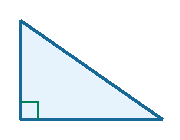
\includegraphics[width=0.34\linewidth]{alternativas/triangulo_retangulo.png}
  \item 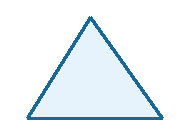
\includegraphics[width=0.34\linewidth]{alternativas/triangulo_acutangulo.png}
  \item 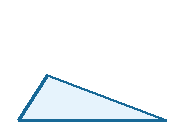
\includegraphics[width=0.34\linewidth]{alternativas/triangulo_obtusangulo.png}
\end{enumerate}

\item Observe o quadrado com uma de suas diagonais traçada.

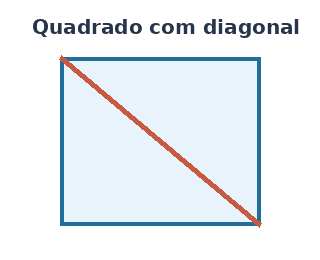
\includegraphics[width=0.56\linewidth]{Q3_TAGFIGURAAQUI.png}

Em quantos triângulos essa diagonal divide o quadrado?
\begin{enumerate}
  \item Um triângulo.
  \item Dois triângulos.
  \item Três triângulos.
  \item Quatro triângulos.
\end{enumerate}

\item Calcule $\sqrt{9}+2^2$.
\begin{enumerate}
  \item $5$.
  \item $6$.
  \item $7$.
  \item $8$.
\end{enumerate}

\end{enumerate}

% Gabarito Matemática:
% 1-b, 2-a, 3-b, 4-c

\end{document}
